\documentclass[11pt,aspectratio=43]{beamer}

\usepackage{amsmath,amssymb}
\usepackage{booktabs}
\usepackage{graphicx}
\usepackage{xcolor}
\usepackage{tikz}
\usetikzlibrary{arrows.meta,positioning,shapes.geometric,calc}

\definecolor{accent}{HTML}{2E75B6}
\definecolor{red2}{HTML}{C0392B}
\definecolor{green2}{HTML}{27AE60}
\definecolor{orange2}{HTML}{E67E22}

\setbeameroption{hide notes}
\setbeamertemplate{navigation symbols}{}
\setbeamersize{text margin left=0.9cm,text margin right=0.9cm}

\setbeamercolor{normal text}{fg=black,bg=white}
\setbeamercolor{frametitle}{fg=black,bg=white}
\setbeamercolor{title}{fg=black}
\setbeamercolor{structure}{fg=black}
\setbeamercolor{alerted text}{fg=accent}
\setbeamercolor{block title}{fg=black,bg=black!10}
\setbeamercolor{block body}{fg=black,bg=black!3}
\setbeamercolor{itemize item}{fg=black}
\setbeamercolor{itemize subitem}{fg=black}

\setbeamerfont{title}{size=\normalsize,series=\bfseries}
\setbeamerfont{frametitle}{size=\normalsize,series=\bfseries}
\setbeamerfont{block title}{size=\small,series=\bfseries}
\setbeamerfont{block body}{size=\small}

\setbeamertemplate{footline}{%
  \leavevmode%
  \hbox{%
    \begin{beamercolorbox}[wd=\paperwidth,ht=2.5ex,dp=1.0ex,rightskip=0.9cm]{author in head/foot}%
      \hfill\insertframenumber
    \end{beamercolorbox}%
  }%
}

\title{Reward Shaping and Training Throughput}
\author{Pulak Mehrotra}
\date{April 2026}

\begin{document}

\begin{frame}[plain]
  \titlepage
\end{frame}

% =========================================================================
% SLIDE 1 — recap
% =========================================================================

\begin{frame}[shrink=3]{Recap: RL beat greedy by spreading load much more effectively.}

  \begin{columns}[T,onlytextwidth]
    \column{0.56\textwidth}
      \begin{center}
      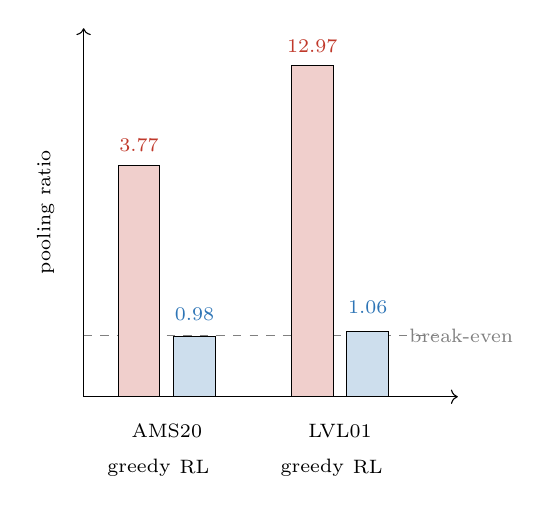
\begin{tikzpicture}[
          x=0.88cm, y=0.78cm,
          lbl/.style={font=\scriptsize, align=center},
          greedy/.style={draw, fill=red2!24},
          rl/.style={draw, fill=accent!24}
      ]
        \draw[->] (0,0) -- (0,6.0);
        \draw[->] (0,0) -- (5.4,0);
        \draw[dashed, gray] (0,1.0) -- (5.1,1.0);
        \node[lbl, rotate=90] at (-0.55,3.0) {pooling ratio};
        \node[lbl, text=gray] at (5.45,1.0) {break-even};

        \draw[greedy] (0.5,0) rectangle (1.1,3.77);
        \draw[rl]     (1.3,0) rectangle (1.9,0.98);
        \draw[greedy] (3.0,0) rectangle (3.6,5.4);
        \draw[rl]     (3.8,0) rectangle (4.4,1.06);

        \node[lbl, text=red2] at (0.8,4.1) {3.77};
        \node[lbl, text=accent] at (1.6,1.35) {0.98};
        \node[lbl, text=red2] at (3.3,5.7) {12.97};
        \node[lbl, text=accent] at (4.1,1.45) {1.06};

        \node[lbl] at (1.2,-0.55) {AMS20};
        \node[lbl] at (3.7,-0.55) {LVL01};
        \node[lbl] at (0.8,-1.15) {greedy};
        \node[lbl] at (1.6,-1.15) {RL};
        \node[lbl] at (3.3,-1.15) {greedy};
        \node[lbl] at (4.1,-1.15) {RL};
      \end{tikzpicture}
      \end{center}

      \begin{center}
        \small Held-out traces, 50 random pod mappings each.
      \end{center}

    \column{0.44\textwidth}
      \begin{center}
      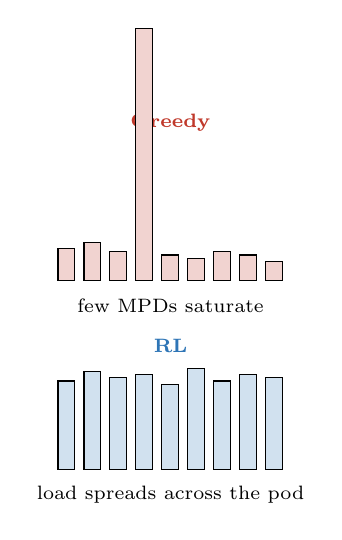
\begin{tikzpicture}[
          x=0.55cm, y=0.40cm,
          greedybar/.style={draw, fill=red2!22},
          rlbar/.style={draw, fill=accent!22},
          lbl/.style={font=\scriptsize, align=center}
      ]
        \node[lbl, text=red2] at (3.0,11.0) {\textbf{Greedy}};
        \foreach \x/\h in {0.4/1.0,1.0/1.2,1.6/0.9,2.2/8.0,2.8/0.8,3.4/0.7,4.0/0.9,4.6/0.8,5.2/0.6} {
          \draw[greedybar] (\x,6.0) rectangle ++(0.38,\h);
        }
        \node[lbl] at (3.0,5.2) {few MPDs saturate};

        \node[lbl, text=accent] at (3.0,3.9) {\textbf{RL}};
        \foreach \x/\h in {0.4/2.8,1.0/3.1,1.6/2.9,2.2/3.0,2.8/2.7,3.4/3.2,4.0/2.8,4.6/3.0,5.2/2.9} {
          \draw[rlbar] (\x,0.0) rectangle ++(0.38,\h);
        }
        \node[lbl] at (3.0,-0.8) {load spreads across the pod};
      \end{tikzpicture}
      \end{center}
  \end{columns}

  \vspace{0.2em}
  \begin{center}
    \small RL is the first policy near break-even on both held-out traces, and it gets there by avoiding the hotspot pattern that greedy creates.
  \end{center}

\end{frame}

% =========================================================================
% SLIDE 2 — recap
% =========================================================================

\begin{frame}{Recap: the remaining problem is reward shaping, not just more training.}

  \begin{columns}[T,onlytextwidth]
    \column{0.60\textwidth}
      \begin{itemize}
        \setlength{\itemsep}{0.8em}
        \item The old reward watched a narrow proxy, so the agent could improve the score without improving final pooling savings.
        \item The newer projected-load reward fixed the worst collapse mode and made training stable.
        \item But savings still plateau around \textbf{1--2\%} early and then stop moving.
        \item So the next bottleneck is \textbf{reward alignment}: what signal should the agent actually optimize?
      \end{itemize}

    \column{0.40\textwidth}
      \begin{block}{Interpretation}
        \small
        The current reward is a \emph{better proxy}, not the true objective.

        \vspace{0.6em}
        Better proxy $\neq$ optimal control signal.
      \end{block}

      \vspace{0.5em}
      \begin{block}{What that means}
        \small
        More timesteps alone are unlikely to fix the plateau.
      \end{block}
  \end{columns}

\end{frame}

% =========================================================================
% SLIDE 3 — reachability
% =========================================================================

\begin{frame}{New reward question 1: how much should reachability constrain the reward?}

  \begin{center}
  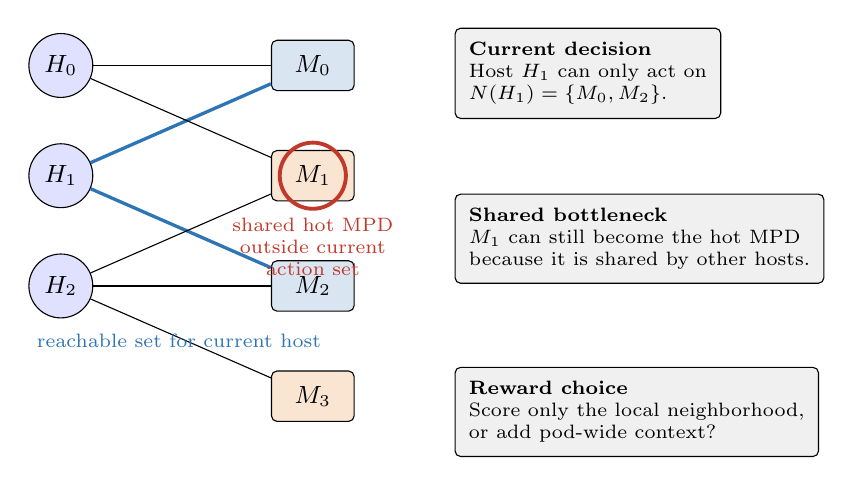
\begin{tikzpicture}[
      x=1cm, y=1cm,
      every node/.style={font=\small},
      host/.style={draw,circle,fill=blue!12,minimum size=0.8cm},
      mpd/.style={draw,rounded corners=2pt,fill=orange2!20,minimum width=1.05cm,minimum height=0.64cm},
      focus/.style={draw,rounded corners=2pt,fill=accent!18,minimum width=1.05cm,minimum height=0.64cm},
      note/.style={draw,rounded corners=2pt,fill=black!6,align=left,font=\scriptsize,inner sep=5pt}
  ]
    \node[host] (h0) at (0,2.4) {$H_0$};
    \node[host] (h1) at (0,1.0) {$H_1$};
    \node[host] (h2) at (0,-0.4) {$H_2$};

    \node[focus] (m0) at (3.2,2.4) {$M_0$};
    \node[mpd]   (m1) at (3.2,1.0) {$M_1$};
    \node[focus] (m2) at (3.2,-0.4) {$M_2$};
    \node[mpd]   (m3) at (3.2,-1.8) {$M_3$};

    \draw[very thick,accent] (h1) -- (m0);
    \draw[very thick,accent] (h1) -- (m2);
    \draw (h0) -- (m0);
    \draw (h0) -- (m1);
    \draw (h2) -- (m1);
    \draw (h2) -- (m2);
    \draw (h2) -- (m3);

    \draw[red2, line width=1.4pt] (m1) circle (0.42);
    \node[note, anchor=west] at (5.0,2.3)
      {\textbf{Current decision}\\Host $H_1$ can only act on\\$N(H_1)=\{M_0,M_2\}$.};
    \node[note, anchor=west] at (5.0,0.2)
      {\textbf{Shared bottleneck}\\$M_1$ can still become the hot MPD\\because it is shared by other hosts.};
    \node[note, anchor=west] at (5.0,-2.0)
      {\textbf{Reward choice}\\Score only the local neighborhood,\\or add pod-wide context?};

    \node[font=\scriptsize, text=accent] at (1.5,-1.1) {reachable set for current host};
    \node[font=\scriptsize, text=red2, align=center] at (3.2,0.1)
      {shared hot MPD\\outside current\\action set};
  \end{tikzpicture}
  \end{center}

\end{frame}

% =========================================================================
% SLIDE 4 — proxy vs actual
% =========================================================================

\begin{frame}{New reward question 2: proxy reward vs.\ actual goal.}

  \begin{columns}[T,onlytextwidth]
    \column{0.50\textwidth}
      \begin{block}{Proxy rewards score each step}
        \centering
        \small post-placement peak\\[0.2em]
        projected load after near-term departures\\[0.2em]
        local or global congestion proxy
      \end{block}

      \vspace{0.5em}
      \begin{block}{Why they help}
        \centering
        dense signal\\
        easier credit assignment\\
        faster learning
      \end{block}

    \column{0.50\textwidth}
      \begin{block}{Actual objective scores the whole episode}
        \[
        \text{pooling\_savings}
        =
        1 -
        \frac{m \cdot \max_j c_j^{\text{peak}}}{D_{\text{pod}}}
        \]
      \end{block}

      \vspace{0.5em}
      \begin{block}{Why it matters}
        \centering
        a step can look locally good\\
        and still create the final episode peak
      \end{block}
  \end{columns}

  \vspace{0.4em}
  \begin{center}
    \small\textbf{Tension:} proxy rewards are learnable, but terminal pooling savings is the quantity we actually care about.
  \end{center}

\end{frame}

% =========================================================================
% SLIDE 5 — optimal gap
% =========================================================================

\begin{frame}[shrink=3]{New reward question 3: can the optimal solver provide a better shaping signal?}

  \begin{columns}[T,onlytextwidth]
    \column{0.58\textwidth}
      \begin{itemize}
        \setlength{\itemsep}{0.7em}
        \item The codebase already has an exact snapshot solver in \texttt{octopus/optimal.py}.
        \item For a given demand vector, it gives the \textbf{lowest achievable peak} under the topology constraints.
        \item That creates an \textbf{optimality-gap} signal:
        \[
          \delta_t = \frac{c_{\max}^{\text{post}} - t^*(s_t)}{D_{\text{pod}}}
        \]
        \item If useful, this is a cleaner shaping term than hand-designed heuristics because it is anchored to a real lower bound.
      \end{itemize}

    \column{0.42\textwidth}
      \begin{block}{Why this is attractive}
        \small
        It tells the policy not just ``did you avoid a hot MPD?'' but ``how far are you from the best possible placement right now?''
      \end{block}

      \vspace{0.5em}
      \begin{block}{Why this is risky}
        \small
        It requires a max-flow solve.
        That makes it the most informative reward candidate and the most expensive one.
      \end{block}
  \end{columns}

\end{frame}

% =========================================================================
% SLIDE 6 — ablation ladder
% =========================================================================

\begin{frame}[shrink=3]{Putting the reward options together.}

  \begin{center}
  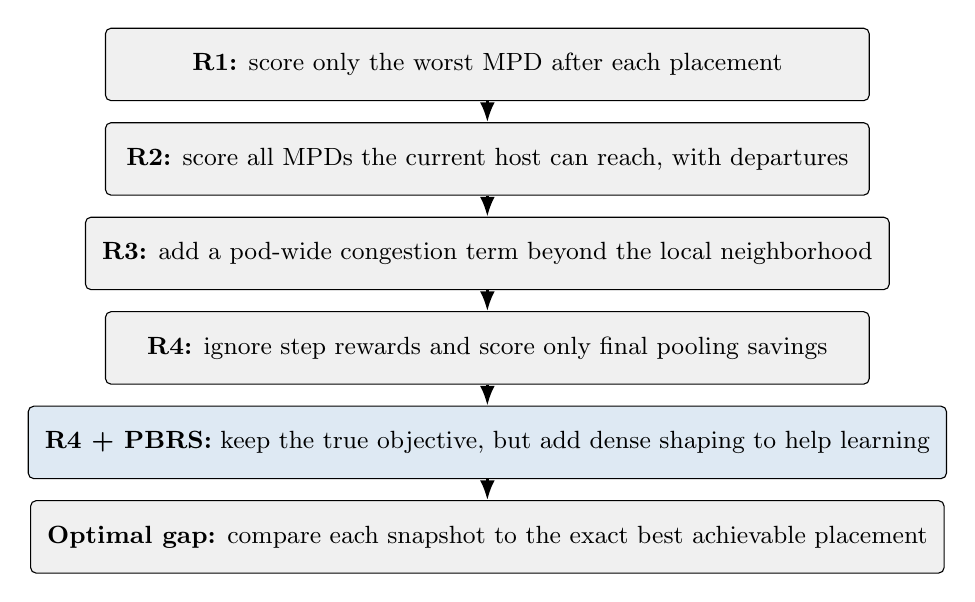
\begin{tikzpicture}[
      every node/.style={font=\small},
      rewardbox/.style={draw,rounded corners=2pt,minimum width=9.7cm,minimum height=0.92cm,align=left,fill=black!6,inner sep=6pt},
      bestbox/.style={draw,rounded corners=2pt,minimum width=9.7cm,minimum height=0.92cm,align=left,fill=accent!16,inner sep=6pt},
      arr/.style={-{Latex[length=2.5mm]}, line width=1.0pt}
  ]
    \node[rewardbox] (r1) at (0,0)
      {\textbf{R1:} score only the worst MPD after each placement};
    \node[rewardbox] (r2) at (0,-1.2)
      {\textbf{R2:} score all MPDs the current host can reach, with departures};
    \node[rewardbox] (r3) at (0,-2.4)
      {\textbf{R3:} add a pod-wide congestion term beyond the local neighborhood};
    \node[rewardbox] (r4) at (0,-3.6)
      {\textbf{R4:} ignore step rewards and score only final pooling savings};
    \node[bestbox] (r5) at (0,-4.8)
      {\textbf{R4 + PBRS:} keep the true objective, but add dense shaping to help learning};
    \node[rewardbox] (r6) at (0,-6.0)
      {\textbf{Optimal gap:} compare each snapshot to the exact best achievable placement};

    \draw[arr] (r1) -- (r2);
    \draw[arr] (r2) -- (r3);
    \draw[arr] (r3) -- (r4);
    \draw[arr] (r4) -- (r5);
    \draw[arr] (r5) -- (r6);
  \end{tikzpicture}
  \end{center}

\end{frame}

% =========================================================================
% SLIDE 8 — timing + systems takeaway
% =========================================================================

\begin{frame}{New rewards turned training into a systems problem.}

  \begin{center}
  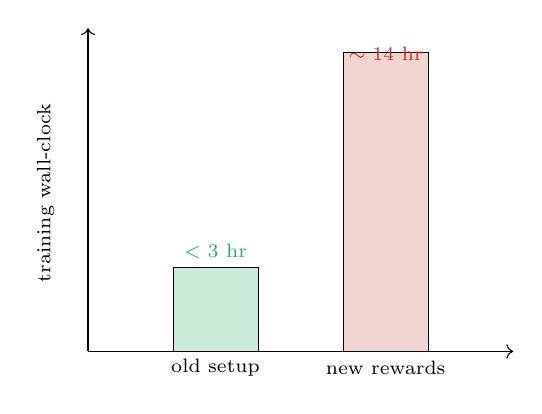
\begin{tikzpicture}[
      x=1.08cm, y=0.38cm,
      old/.style={draw, fill=green2!25},
      new/.style={draw, fill=red2!22},
      lbl/.style={font=\scriptsize, align=center}
  ]
    \draw[->] (0,0) -- (0,10.8);
    \draw[->] (0,0) -- (5.0,0);
    \draw[old] (1.0,0) rectangle (2.0,2.8);
    \draw[new] (3.0,0) rectangle (4.0,10.0);
    \node[lbl] at (1.5,-0.55) {old setup};
    \node[lbl] at (3.5,-0.55) {new rewards};
    \node[lbl, text=green2] at (1.5,3.35) {$<3$ hr};
    \node[lbl, text=red2] at (3.5,9.95) {$\sim 14$ hr};
    \node[lbl, rotate=90] at (-0.5,5.3) {training wall-clock};
  \end{tikzpicture}
  \end{center}

  \vspace{0.15em}
  \begin{block}{Takeaway}
    \footnotesize
    \begin{itemize}
      \setlength{\itemsep}{0.2em}
      \item Rewards became more informative, but experiment turnaround became much slower.
      \item The main blocker is throughput: each reward iteration now carries substantial wall-clock cost.
    \end{itemize}
  \end{block}

\end{frame}

% =========================================================================
% SLIDE 7 — slow
% =========================================================================

\begin{frame}{Quick profile: where time goes and what we can remove.}

  \begin{columns}[T,onlytextwidth]
    \column{0.56\textwidth}
      \begin{center}
      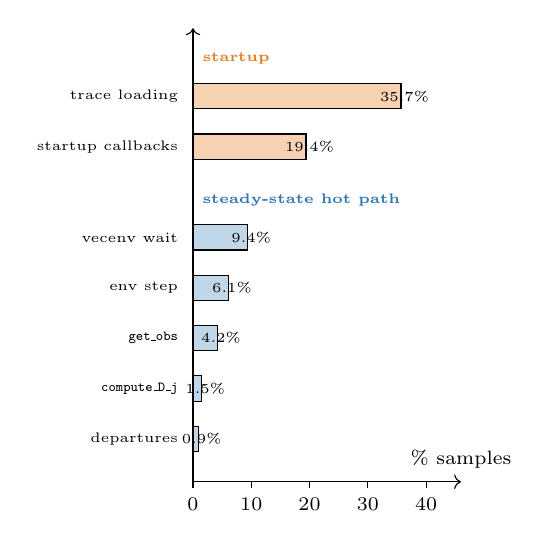
\begin{tikzpicture}[
          x=0.074cm, y=0.64cm,
          lbl/.style={font=\tiny, align=right},
          pct/.style={font=\tiny, align=left},
          grp/.style={font=\tiny\bfseries, align=left},
          barS/.style={draw, fill=orange2!35},
          barH/.style={draw, fill=accent!30}
      ]
        % Axes
        \draw[->] (8,0) -- (54,0);
        \draw[->] (8,0) -- (8,9.0);
        \node[font=\scriptsize] at (54,0.45) {\% samples};

        % Tick marks
        \foreach \x in {0,10,20,30,40} {
          \draw (8+\x,0) -- (8+\x,-0.12);
          \node[font=\scriptsize] at (8+\x,-0.45) {\x};
        }

        % Group label: startup (amortizable)
        \node[grp, text=orange2, anchor=west] at (8,8.4) {startup};

        \draw[barS] (8,7.4) rectangle (43.7,7.9);
        \node[lbl, anchor=east] at (7.1,7.65) {trace loading};
        \node[pct] at (44.3,7.65) {35.7\%};

        \draw[barS] (8,6.4) rectangle (27.4,6.9);
        \node[lbl, anchor=east] at (7.1,6.65) {startup callbacks};
        \node[pct] at (28.0,6.65) {19.4\%};

        % Group label: steady-state hot path
        \node[grp, text=accent, anchor=west] at (8,5.6) {steady-state hot path};

        \draw[barH] (8,4.6) rectangle (17.4,5.1);
        \node[lbl, anchor=east] at (7.1,4.85) {vecenv wait};
        \node[pct] at (18.0,4.85) {9.4\%};

        \draw[barH] (8,3.6) rectangle (14.1,4.1);
        \node[lbl, anchor=east] at (7.1,3.85) {env step};
        \node[pct] at (14.7,3.85) {6.1\%};

        \draw[barH] (8,2.6) rectangle (12.2,3.1);
        \node[lbl, anchor=east] at (7.1,2.85) {\texttt{get\_obs}};
        \node[pct] at (12.8,2.85) {4.2\%};

        \draw[barH] (8,1.6) rectangle (9.5,2.1);
        \node[lbl, anchor=east] at (7.1,1.85) {\texttt{compute\_D\_j}};
        \node[pct] at (10.1,1.85) {1.5\%};

        \draw[barH] (8,0.6) rectangle (8.9,1.1);
        \node[lbl, anchor=east] at (7.1,0.85) {departures};
        \node[pct] at (9.5,0.85) {0.9\%};
      \end{tikzpicture}
      \end{center}

      \begin{center}
        \scriptsize \textit{py-spy, main process, short probe (2k steps).}
      \end{center}

    \column{0.44\textwidth}
      \begin{block}{Startup $\rightarrow$ cache it}
        \small
        Trace loading + callbacks dominate short ablation runs.\\
        Fix: \textbf{multi-trace precompute cache}, reused across \texttt{reset()}.
      \end{block}

      \vspace{0.4em}
      \begin{block}{Hot path $\rightarrow$ vectorize it}
        \small
        \texttt{get\_obs}, \texttt{compute\_D\_j}, departures all walk \texttt{mpd\_vm\_allocs} in Python.\\
        Fix: \textbf{flat-array MPD state}, NumPy hot kernels.
      \end{block}
  \end{columns}

\end{frame}

% =========================================================================
% SLIDE 9 — redesigned architecture
% =========================================================================

\begin{frame}{Proposed plan: attack the two bottlenecks directly.}

  \begin{center}
    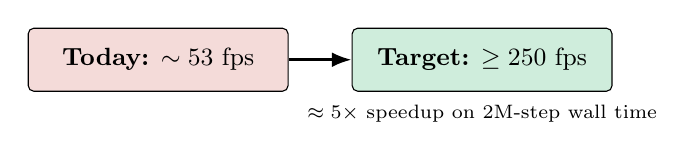
\begin{tikzpicture}[
        baseline=(cur.base),
        curbox/.style={draw,rounded corners=2pt,fill=red2!18,
                       minimum width=3.3cm,minimum height=0.8cm,align=center,inner sep=4pt},
        tgtbox/.style={draw,rounded corners=2pt,fill=green2!22,
                       minimum width=3.3cm,minimum height=0.8cm,align=center,inner sep=4pt},
        arr/.style={-{Latex[length=2.5mm]}, line width=1.0pt}
    ]
      \node[curbox] (cur) {\small\textbf{Today:} $\sim 53$ fps};
      \node[tgtbox, right=0.8cm of cur] (tgt) {\small\textbf{Target:} $\geq 250$ fps};
      \draw[arr] (cur) -- (tgt);
      \node[font=\scriptsize, below=0.05cm of tgt, anchor=north] {$\approx 5\times$ speedup on 2M-step wall time};
    \end{tikzpicture}
  \end{center}

  \vspace{0.2em}

  \begin{columns}[T,onlytextwidth]
    \column{0.99\textwidth}
      \begin{center}
      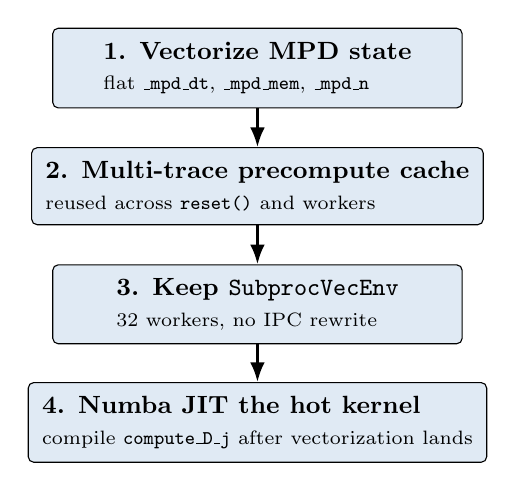
\begin{tikzpicture}[
          every node/.style={font=\small},
          planbox/.style={draw,rounded corners=2pt,fill=accent!15,
                          minimum width=5.2cm,minimum height=0.9cm,align=left,inner sep=5pt},
          optbox/.style={draw,rounded corners=2pt,fill=black!6,
                         minimum width=5.2cm,minimum height=0.9cm,align=left,inner sep=5pt},
          arr/.style={-{Latex[length=2.5mm]}, line width=1.0pt}
      ]
        \node[planbox] (s1) at (0,2.7)
          {\textbf{1. Vectorize MPD state}\\
           \scriptsize flat \texttt{\_mpd\_dt}, \texttt{\_mpd\_mem}, \texttt{\_mpd\_n}};
        \node[planbox] (s2) at (0,1.2)
          {\textbf{2. Multi-trace precompute cache}\\
           \scriptsize reused across \texttt{reset()} and workers};
        \node[planbox] (s3) at (0,-0.3)
          {\textbf{3. Keep \texttt{SubprocVecEnv}}\\
           \scriptsize 32 workers, no IPC rewrite};
        \node[planbox] (s4) at (0,-1.8)
          {\textbf{4. Numba JIT the hot kernel}\\
           \scriptsize compile \texttt{compute\_D\_j} after vectorization lands};

        \draw[arr] (s1) -- (s2);
        \draw[arr] (s2) -- (s3);
        \draw[arr] (s3) -- (s4);
      \end{tikzpicture}
      \end{center}

    \column{0.01\textwidth}
      % \begin{block}{Why this, not GPU}
      %   \small
      %   Env is event-driven with variable-length per-MPD state.
      %   CPU + NumPy fits that shape; a GPU-native env would mostly move Python loops through \texttt{.item()} calls.
      % \end{block}

      \vspace{0.4em}
      % \begin{block}{Validation gates}
      %   \small
      %   \begin{itemize}
      %     \setlength{\itemsep}{0.3em}
      %     \item Report FPS and wall-clock per 200k steps.
      %     \item Matched-seed curve overlap vs. baseline.
      %     \item No regression on pooling savings.
      %   \end{itemize}
      % \end{block}
  \end{columns}

\end{frame}

\end{document}
